%!TEX root = /Users/markelikalderon/Documents/Git/timaeus/timaeus.tex

\chapter{The Anatomy of Tripartition} % (fold)
\label{cha:the_flesh_and_the_mortal_soul}

\section{The Methodological Dilemma Revisited} % (fold)
\label{sec:the_methodological_dilemma_revisited}

Recall that Timaeus inaugurates his discussion of the \emph{pathēmata} with a methodological dilemma (61c4–d5). The \emph{pathēmata}, affections of the corporeal instruments of \emph{aisthēsis}, are contrasted with two other things. Specifically they are contrasted with the origin of the flesh and things pertaining to it, on the one hand, and the mortal parts of the soul, on the other. The problem is twofold. First, one cannot adequately account for the \emph{pathēmata} having to do with \emph{aisthēsis} without accounting for the origin of the flesh and things pertaining to it and the mortal part of the soul. But second, one cannot account for the origin of the flesh and things pertaining to it and the mortal parts of the soul without accounting for the \emph{pathēmata} having to do with \emph{aisthēsis}. The problem is not one of mutual entailment or that these subject matters somehow presuppose one another directly. The problem is rather that an account of either subject matter each presupposes \emph{aisthēsis} with the consequence that an account of each must make reference to the other. Hence the methodological dilemma: Timaeus cannot account for either without reference to the other, but it is impossible to give an account of both subjects at once. Timaeus solution is to first account for the \emph{pathēmata} (61d–68d) and then subsequently account for the origin of the flesh and things pertaining to it (73b1ff) and the mortal parts of the soul (69c5ff). 

We have already discussed Timaeus' account of the \emph{pathēmata} common to the body as a whole and peculiar to particular parts of the body (chapters~\ref{cha:common_pathemata} and \ref{cha:peculiar_pathemata}). In the present chapter we shall discuss the origin of the flesh and things pertaining to it and the mortal parts of the soul. Unfortunately not the whole of it. Our approach will be selective. The selection is subservient to two goals. First, I want to learn what I can about how the methodological dilemma is resolved from this discussion. As audition is the clearest case where further insight is shed on a perceptual power, it is natural, as well, to focus on this. Second, I want to learn what the mortal soul is and how it acts as a principle of vital activity.

Earlier, when I said it was unfortunate that we are not in a position to discuss the whole of Timaeus' account of the flesh and the mortal soul, one may be forgiven for hearing a hint of irony. None was intended. The significance of Timaean anatomy is underappreciated. For just consider the context. Socrates the day before, on the occasion of the Panathenaea, has given a speech on the topic of the \emph{Republic} and requests that the return speeches he is now owed portray Socrates' ideal city in action. Critias proposes that a secret history, passed down in his family, of ancient Athenians fighting a war with Atlantis over the Mediterranean would serve this purpose. This history will be delivered only after Timaeus' cosmology. What is the connection? The Cosmos is only completely perfected when there are mortal living beings embodied and embedded within it. Anthropogony is required to perfect the Cosmos by making it better resemble the intelligible Living Being upon which it was modeled by the Demiurge. The intelligible Living Being is comprehensive. It contains within it all other intelligible living beings. In order for the sensible Cosmos to be comprehensive, it must contain within it all other sensible living beings. As a consequence of divinely ordained embodiment, mortal souls not only have an immortal part, which the Demiurge addressed in delivering the Laws of Destiny, but now have a mortal part as well. There are two parts of the mortal soul, the spirited part, and the appetitive part. So Timaeus seems to subscribe to a tripartite psychology, though there are differences between the Timaean account and the accounts found in the \emph{Republic} and the \emph{Phaedo}. Thus, as \citet[496]{Taylor:1928qb} observes, the tripartite psychology of the \emph{Republic} is not explicitly linked to anatomy the way it is in the \emph{Timaeus}. Nevertheless, Timaeus retains the city--soul analogy. Moreover, the moral psychology determined by his anthropogony, required for the perfection of the Cosmos, is the moral psychology of the Athenian heroes who stopped the invasion of the Mediterranean by Atlantis. It is only if the actions of the Athenians are sufficiently like the actions of Socrates' ideal city will the return \emph{logoi} meet with his approval. And in order for Timaeus' speech to contribute to this collective effort, the actions of the Athenian heroes must be explicable in terms of the moral psychology dictated by his anthropogony. And these are bound up with commitments concerning the flesh and the mortal soul.

A vivid example of the ethical significance of Timaean anatomy involves audition. We are providentially provided ears to hear with to correct the revolutions of the immortal soul disrupted as a result of being embodied and embedded in an environment with strong powers and so subject to the irrational linear motion of \emph{aisthēsis}. In listening to music or rational speech with rational attentiveness, the revolutions of the soul have a tendency to align with the revolutions of our elder sister, the World Soul. While we have been told that sound impacts upon the brain and the blood through the ears and causes a motion from the head to the region of the liver, the rational effects of rational attentive listening have yet to be explained. These, however, become explicable once we understand the ethical function of the liver. So our knowledge of Divine Providence is incomplete without detailed anatomical knowledge of the liver (a lowly, ignoble organ confined with the beasts of appetite to a manger far enough for their din to be unable to reach the acropolis from which the rational part of the soul rules and issues sovereign commands).

% section the_methodological_dilemma_revisited (end)

\section{Tripartition in the \emph{Timaeus}} % (fold)
\label{sec:tripartition_in_the_emph_timaeus}

The Demiurge generates the immortal soul in the hypercosmic \emph{kratēr} mixing together indivisible and divisible Being, Sameness, and Difference. Souls are individuated from this soul mixture by the Demiurge apportioning parts of this mixture and mounting them in stars as in vehicles. This immortal part is joined to a mortal part as a result of embodiment. The mortal part of the soul is the principle of embodied vital activity. The three parts of the soul consist in the immortal part, the rational part of the soul, and the two parts of the mortal part, the spirited and appetitive parts. These share the body as a vehicle, as drivers rather than passengers, and are said to cohabit that body and so come to share a common household or perhaps more aptly a common \emph{polis} (Timaeus shifts freely between domestic and civic imagery). The three parts of the soul are associated with different regions of the body. For each part of the mortal soul, Timaeus will single out a primary and secondary organ. His anatomical descriptions are rough if accurate (especially given the state of anatomical knowledge in the 5th century B.C.E). What is striking is the language he uses to describe their relative locations and the functions that he assigns to them. 

First, the language that Timaeus uses to describe the locations of the parts of the soul is striking. Taken collectively they describe a \emph{polis}. 

The immortal part of the soul, the rational part, is in the head since the roundness of the skull resembles the shape of the Cosmos and so may accommodate the soul's revolutions. In the \emph{Republic}, the rational part was described as the acropolis of the soul, but in Timaeus' hands the rational part is an occupant of the acropolis \citep[81]{Price:1995hc}. An acropolis is a fortified city within a city, usually on a hill. (The Greek from which ``acro-'' derives means high, and so acropolis suggests a city on high.) Just as the Circle of the Same has sovereignty over the Circle of the Different, the rational part of the soul, comprised of these, has sovereignty over the mortal parts of the soul and the body that it animates. From its shining acropolis, the rational part of the soul issues discursive commands that may be heard and heeded by the mortal soul.

The mortal part of the soul is separated from the immortal part by an isthmus. An isthmus is a narrow land bridge bounded by water joining two larger bodies of land. So we are to imagine the acropolis on a hill set in the water overlooking the rest of the \emph{polis} spread out beneath it on the mainland to which it is bound by a narrow isthmus. \citet[500]{Taylor:1928qb} suggests that Plato might have had Syracuse in mind, a city with which he was familiar (see the Platonic Letters). If correct, then the island set apart from the mainland is modeled on Ortygia. While separated in this way, this is consistent with their being some line of communication between the acropolis and the rest of the \emph{polis}, for discursive commands are issued from the acropolis and heard and heeded by the mortal soul. 

The spirited part of the soul is housed in the upper thorax just beyond the isthmus that separates it from the immortal soul. Located there is the barracks of the guardians, the heart. The barracks are located just beyond the isthmus so that it may better hear and heed the discursive commands of the acropolis. Spirit is portrayed as fulfilling the role of the guardians, attacking both external and internal enemies.

The appetitive part is portrayed as unruly beasts confined to a manger where they are safely bound. The manger is located far away from the acropolis so as to be out of earshot, at least normally. Being free from the turmoil and din of unruly beasts allows the supreme soul, the rational immortal soul, to take its own counsel in peace concerning what is best for one and all. Perhaps the mirror-like liver is a still pool adjacent to the manger. It is more likely, though, that Timaeus has merely shifted the imagery to a domestic interior (the significance of which shall emerge in sequel).

Timaues has provided us with a political topology of the soul. Each part of the soul being located where the appropriate class of people are located in Socrates' ideal city.

It is not just the political topology of his descriptions that is striking, but the functions that he assigns to the primary and secondary organs associated with the two mortal parts of the soul. While Timaeus provides reasonably accurate anatomical descriptions of these organs, he is not at all concerned with their primary biological function. Instead he assigns them ethical functions that correspond to the functions of the different classes in the ideal city. Or more specifically, the ethical functions are assigned to the primary organs and the secondary organs have an auxiliary function in aiding and maintaining the primary organ. The rational part, of course, rules. The heart is the primary organ associated with the spirited part, but Timaeus does not here mention the role of the circulation of blood in nutrition and respiration, but focuses, instead, on the boiling of the blood in anger when reason communicates some injustice. The lungs, the secondary organs associated with spirit, serve to cool the heart when it becomes overheated. Though Timaeus has an elaborate theory of respiration, no mention of respiration is made here. Instead, the lungs play the regulatory role that they do in order to maintain the heart and so that it may continue to execute its ethical function. From the biological perspective, one might have expected the stomach to be the primary organ associated with the appetitive part given its role in nutrition, and though Timaeus provides an account of the stomach and digestion more generally, Timaeus does not here mention nutrition. Instead, the liver is the primary organ associated with the appetitive part. Since appetite cannot understand the discursive demands of reason, the liver is providentially provided to compensate for this. The liver may not be able to receive discursive content that it can understand but thanks to its smooth surface it may receive visual content in the form of images reflected on its surface. Reason uses these images to control the mortal part of the soul when it otherwise refuses to heed its command. Moreover, the appetitive part of the soul is further providentially accommodated by the liver being the source of divination.

% section tripartition_in_the_emph_timaeus (end)

\section{The Number of Demiurgic Agency} % (fold)
\label{sec:the_number_of_demiurgic_agency}

In the \emph{proemium}, as Timaeus invokes the Gods, he first does so in the singular and then in the plural. We wondered whether this was an anticipatory trace of a puzzling usage that we find especially prominent in this part of Timaeus' speech. Specifically, Timaeus, at this point, has the tendency to slide freely between singular and plural in describing demiurgic activity (\citealt[280]{Cornford:1935fk}, \citealt[169]{Grube:1935ad}, \citealt[608]{Cherniss:1944aa}). More specifically, \emph{theos} (god, in the singular), \emph{theoi} (gods, in the plural), and \emph{to theion} (the divine) are increasingly used interchangeably. In some cases, the same demiurgic activity is described indifferently in the singular and plural (44e--45a, 46e8--47c5, 71a, 75b--d, 77a3, 80e1). More striking still is Timaeus tendency to use the singular \emph{theos} when, the activity is question is collective and so plural (71a7, 71e3, 74d6, 78b2, 80e1, 92a3). The puzzle posed by such usage might be resolved by arguing that the problematic occurrences of \emph{theos} are meant generically, and so are used like \emph{to theion}. If \emph{theos} is meant generically, then despite being grammatically singular, its occurrence does not designate a particular deity. While this may plausibly be argued in some cases, I doubt that it can for all. 

Timaeus using \emph{theos} to refer to what is, by Timaeus' lights, the activity of the Young Gods might suggest that he is not after all serious about this aspect of Timaean theology. Perhaps in these passages the mask is slipping and Timaeus is quietly dropping the pretense that a distinction should be marked between a superior deity, the Demiurge, and inferior deities, the Young Gods. The usage of \emph{theos} as the subject of collective activity is puzzling, but it is insufficiently puzzling to warrant, by itself, skepticism about this central contrast in Timaean theology.

How else might this puzzling usage be understood?

Let us consider one such occurrence that will be presently relevant. Appetite does not understand reason though it has a share in the perception of reasons. To compensate for this inability, God (\emph{theos}) constructed the liver. Notice that the agent of providence is God in the singular. This, however, is the Young Gods' task. Anthropogony proceeds through divine rational cooperation. The Demiurge creates the immortal part of mortal beings, to which the Young Gods weave the mortal parts to. The Young Gods are charged as well with the generation of these mortal parts, namely, the body composed of corporeal material borrowed from the Cosmos, on the one hand, and the mortal soul, on the other. The construction and placement of the liver is clearly the assigned responsibility of the Young Gods. So why is God in the singular credited with the fulfillment of that responsibility? 

The Young Gods have rationally assented to assist the Demiurge in completing the Cosmos with the generation of mortal beings. The Young Gods assistance is crucial, since the Demiurge is only capable of creating immortal beings. So why attribute their work to the Demiurge incapable of it? Anthropogony, though a cooperative rational activity, remains nonetheless determined by the will of a benevolent and ungrudging Demiurge. It is because the benevolent and ungrudging Demiurge intends to generate the best Cosmos that he intends that it best resemble the comprehensive intelligible Living Being upon which it is modeled. In order for the sensible Cosmos to be like the intelligible Living Being it must itself be comprehensive and so contain within itself all other sensible living beings. And so the Cosmos must contain within itself mortal beings. Perhaps it is the explanatory priority of the Demiurgic will that is expressed by crediting the fulfillment of a collective task to God in the singular. Perhaps, Timaeus, in these contexts, is drawing our attention to the \emph{aitia} rather than the \emph{sunaitia} of anthropogony.


% section the_number_of_demiurgic_agency (end)

\section{Reason} % (fold)
\label{sec:reason}

Recall Timaeus' account of the generation of the head. The Young Gods bound the divine revolutions (\emph{theias periodous}), the revolutions of the Circles of the Same and the Different, within a spherical body. This spherical body is an imitation of the spherical body of the Cosmos. There is, however, a notable difference with respect to the soul–body union. Whereas the body of the Cosmos is bound within the World Soul, the soul of mortal beings is bound within the spherical body. This spherical body is called the “head”. Like the body of the visible god, it is divine, and given its divine status it reigns over the other parts of the mortal being which serve it.

The theme of containment continues in the present passage in a number of guises. The immortal soul is in the body as in a vehicle, as a driver finally not merely as a passenger (though this contrast has yet to be explained). This is a corporeal image of containment. Think of the way in which a carriage or chariot contains its occupants, be they passengers or driver. Moreover, the immortal soul is contained within the head. As we shall see it is bound to the marrow made of the finest triangles within the circular head. The imortal soul is represented as the occupant of an acropolis and so as contained within it. 

The image of the acropolis is worth dwelling on (see figure~\ref{acropolis}). Again, an acropolis is a fortified city within a city, usually on a hill or otherwise elevated, that is the seat of political power. The divine revolutions are sovereign over the mortal soul and the body that it animates. The immortal soul issues discursive commands that are heard and heeded by the mortal soul. It is apt then that the immortal soul, given its divine status and sovereignty over the mortal, should be seated in an acropolis. Two further features of an acropolis are worth dwelling on---that they are fortified and that they are elevated.

\begin{figure}[htbp]
     \centering
         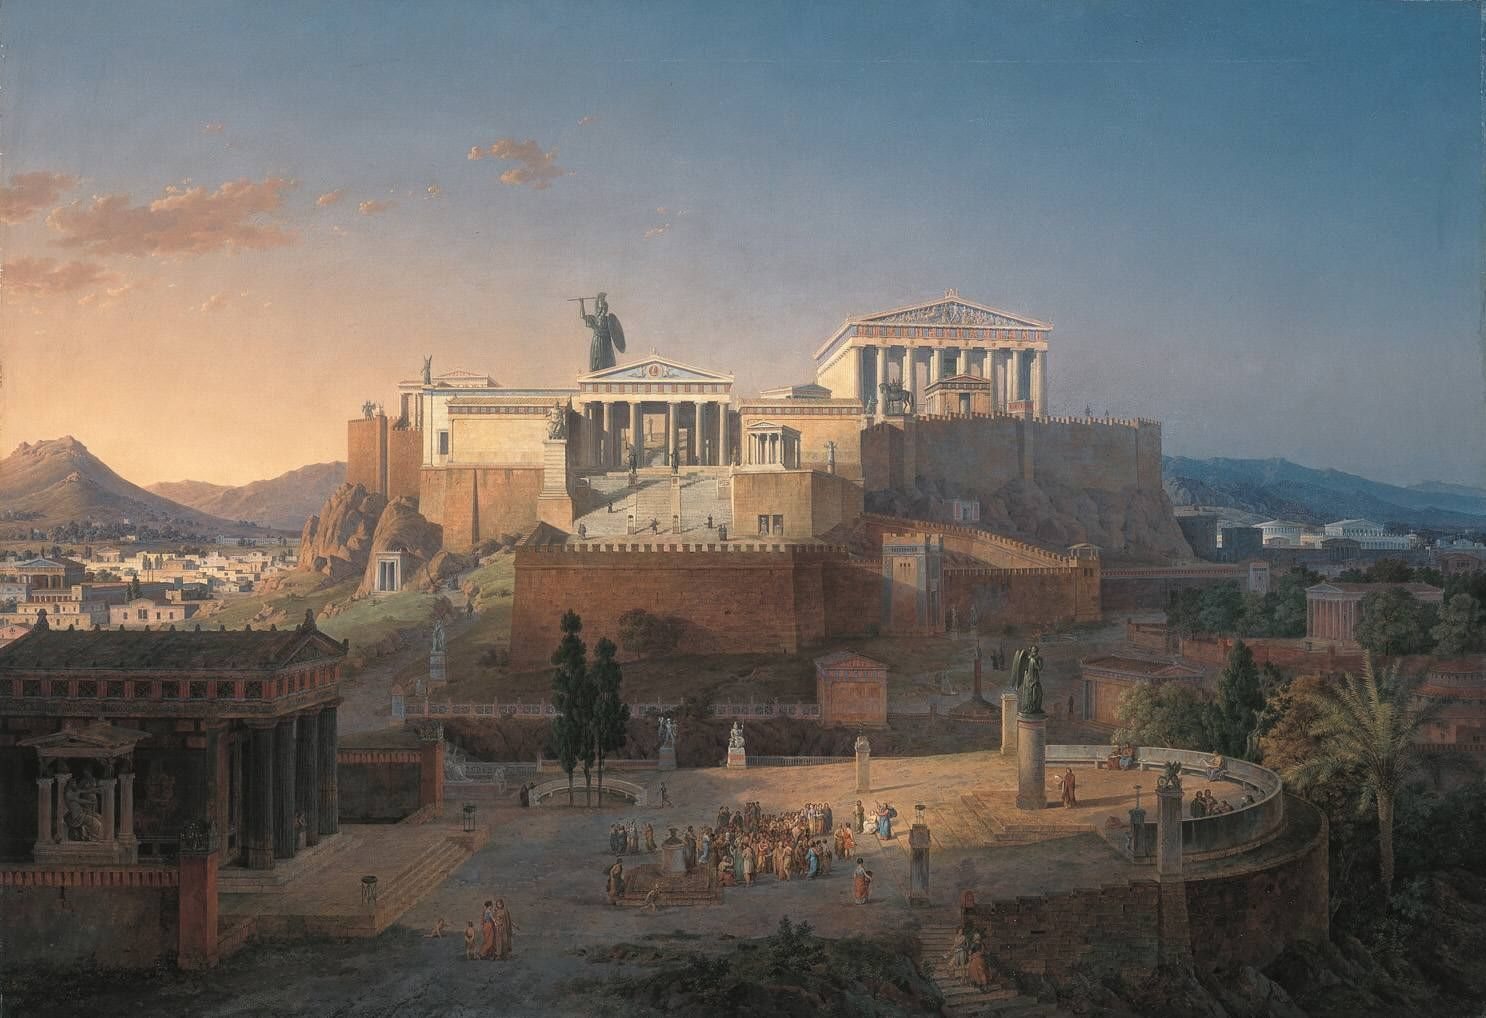
\includegraphics[scale=0.20]{graphics/Akropolis_by_Leo_von_Klenze.jpg}
     \caption{\emph{Acropolis of Athens}, Leo von Klenze, 1846, Neue Pinakothek, Munich}
     \label{acropolis}
\end{figure}

First, an acropolis is fortified. As the seat of political power it is prudential that it is. The sovereign divine revolutions are occupants of an acropolis and so are occupants of a fortified position. The skull of the head is the fortification of the immortal soul that is bound within. The thickness of the skull, and so the effectiveness of the fortification, is carefully balanced to optimize the intelligence of mortal beings. The thicker the skull, the better fortified, but the less room there is for marrow with which to bind the divine revolutions. The immortal soul is immortal. Strictly speaking, the fortification of the skull defends not the immortal soul but what binds it to the marrow of the skull. 

Second, an acropolis is typically located in an elevated position. There may be a number of reasons in play. In being elevated, the acropolis is closer to the divine and the intelligible, the source of its occupants' political authority. Being elevated is also a visible symbol of the political authority invested in the occupants of the acropolis. Finally, being elevated is an aspect of its extended fortification, in that an elevated position is easier to defend. At least the first two reasons are relevant to Timaeus' speech and possibly the third. Let us consider these in turn.

Perhaps the head is elevated so that it may be closer to the divine and the intelligible. The head, the acropolis of the immortal soul, is elevated in humans as opposed to beasts with four legs whose heads are directed downwards, towards the earth (91e). By contrast, the human head, in being elevated, may look, instead, to the Heavens and the intelligible. The head raises us up to kindred Heaven. In this regard, we are not like an earthly plant but a heavenly plant (90a). The Sun illuminates the wanderers so that we may see their motion (46e) and learn the art of number and perhaps even philosophy. The revolutions of the Heavens are divine thought made visibly manifest. In rationally attending to these in the right sort of way, we may perfect ourselves by assimilating to the divine. We are drawn to the divine and the intelligible through the Sun's illumination and this thanks, in part, to the Young Gods providentially providing the head with an elevated position in the human body. 

Timaeus hails from Locrus, but Plato having Timaeus describe the head in these terms may be the expression of a broader Athenian rationalism. Consider the following dramatic incident from Euripides' \emph{Heracles} (see figure~\ref{heracles}). Acting on Hera's orders, Iris has Madness drive Heracles in a frenzy in which kills his wife and children. Theseus, who Heracles had rescued from Hades, encounters Heracles grieving with his father, Amphitryon. Amphitryon entreats Heracles to throw the mantle from his eyes and look to the Sun (\emph{Heracles} 1204--5). And Theseus, in a moving gesture of friendship, declares that he has no fear of pollution, and demands that Heracles unveil himself and look up (\emph{Heracles} 1225). Unveiling and looking up is to rationally attend to one's circumstance, and this is ethically significant. To fail to do so is ignoble even should one's circumstance be terrible as is the tragic situation that Theseus finds Heracles in. Rationally attending to one's circumstance is a kind of acceptance, and the noble soul endures divinely ordained misfortune and does not refuse them (\emph{Heracles} 1225). Euripides, like Timaeus, emphasizes that the head should be elevated, and there is a similar play with the divine, the intelligible, and the Sun's illumination. I am not claiming any specific influence here (though on the influence of Euripides on Plato see \citealt{Sansone:1996ux}). Rather, I claim only that Plato, in having Timaeus place the divine revolutions in the shining acropolis, gives specific expression to a broader Athenian rationalism.

\begin{figure}[htbp]
     \centering
         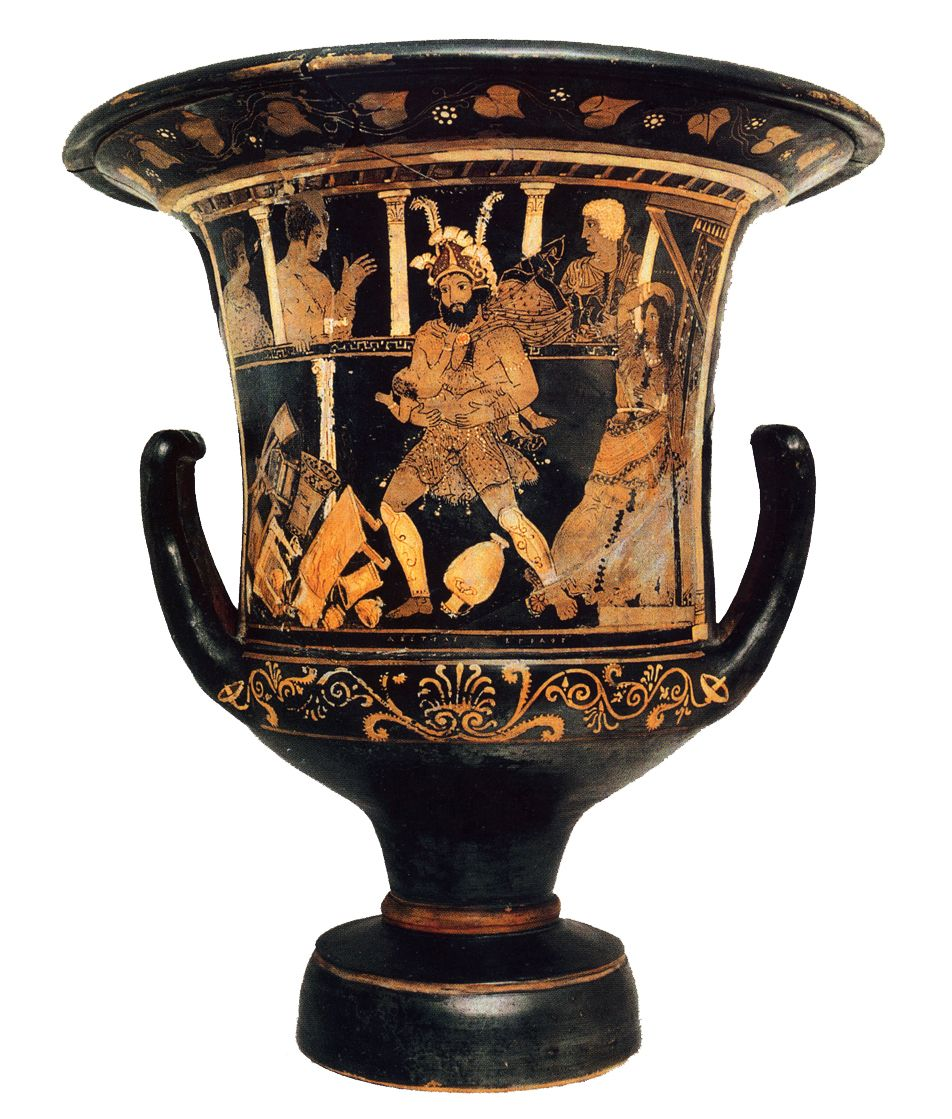
\includegraphics[scale=0.25]{graphics/heracles.jpg}
     \caption{\emph{Krater of the Madness of Heracles}, Calyx type, Side A, between 350 and 320 BCE, Museo Arqueológico Nacional, Madrid}
     \label{heracles}
\end{figure}

Perhaps the head is elevated as the expression of the political authority of its occupant. The immortal soul is divine and so suited to rule over the mortal soul and the body that it animates, and its being seated in the acropolis is an expression of its political authority. In demanding that Heracles raise his head, Theseus can be understood as exhorting Heracles to exercise rational control over his grief and regain his noble authority overthrown by grievous tragedy. The divine revolutions have political authority over the mortal soul and the body that it animates, and that its fortification is elevated is a visible expression of that political authority. 

Perhaps the head is elevated since an elevated position is easier to defend. If the third reason is in play as well, then elevation is an extended fortification. The head may be elevated to make it easier to defend from, say, low lying attacks from beasts on all fours. Thus, a dog may bite your hand or leg, but as long as you are standing, it cannot bite your head.

These three reasons are distinct, if complementary. I am inclined to believe that at least the first two are in play in Timaeus' speech.  I hesitate to endorse the third reason since Timaeus does not make it explicit. Like the utility of sight in navigating a complex environment, the benefit of an elevated position being easier to defend, if genuine, goes unmentioned.

There are two further aspects of the acropolis' fortification. Both may be described as parts of the extended fortification of the acropolis.

First, not only is the immortal soul bound in marrow encased in a hard skull in an elevated position, but it is separated from the region of the body occupied by the mortal soul. The head is separated from the trunk of the body by a narrow isthmus, the neck. If the hardness of skull and elevated position are meant to fortify against external attacks, the separation by means of a narrow isthmus is meant to defend against internal disruptions. Think of the disruptions of the cognitive revolutions occasioned by the \emph{pathēmata} of linear \emph{aisthēsis} in the shock of embodiment. While the immortal soul is divine, the source of these disruptions is corporeal, and Timaeus represent these as a form of pollution. (A potential point of contrast with Theseus who claims the divine does not fear pollution from mortals, but this is not the usual Greek view, and perhaps this is nothing more than a comforting lie directed towards the still grieving Heracles, \emph{Heracles} 1230.)

Second, just past the isthmus is stationed a barracks of guardians, the heart. The spirited part of the soul is the most receptive to the discursive commands of the divine revolutions. The heart is located just beyond the isthmus, in part, to better hearken to sovereign command. The heart may become inflamed because of an injustice perceived by reason. The source of the injustice may be internal as well as external and so, importantly, the heart plays a policing role, as well, in keeping the unruly aspects of the appetitive soul in line so that they may not disrupt the divine revolutions of the soul. In these respects, in guarding against external and internal disruptions of the divine revolutions, the heart is part of the extended fortification of the acropolis.

% section reason (end)

\section{Spirit} % (fold)
\label{sec:spirit}

Just as the immortal part of the soul is separated from the mortal part by means of a narrow isthmus, the mortal part is itself divided. The mortal part of the soul is located in the thorax. The better part is separated from the worse part. The architectural imagery persists but has shifted from a civic to a more domestic setting. Timaeus asks us to envision the better part separated from the worse part as a division separating the men's chambers from the women's chambers, perhaps by means of a screen. The imagery of containment persists. The better and worse parts of the mortal soul are contained as occupants in divided chambers. This division is the midriff or perhaps the diaphragm more specifically. In a passage overtly influenced by Timaeus, Aristotle will deliberately echo Timaeus in describing the diaphragm as a partition (\emph{De partibus anamalium} 3.9 672b). Timaeus' description of this biological detail in terms of a common domestic setting signals, by way of contrast with the divine splendor of the sovereign acropolis, that we have moved from the ruler to the ruled. There may be another way in which the civic and domestic imagery interact. In portraying the broader \emph{polis}, where the majority of the population lives and works, as a domestic household Timaeus echoes and elaborates an aspect of the ideal city---that the citizens of the city are encouraged to think of themselves as family. And, as Timaeus elaborates, since the citizens are family, within the \emph{polis} they are occupants of a common domestic household. Furthermore, the domestic setting, a household separated into two chambers by means of a screen, must be read as a description of the broader \emph{polis} since civic structures of that \emph{polis}---the barracks of the guardians, the manger---are located within these chambers.

Spirit, the better part of the mortal soul, is housed in the men's chambers. These are nearer to the isthmus bordering the grounds of the acropolis. So the men's chambers in which the better part of the mortal soul is housed is the upper thorax, above the midriff or diaphragm. (For reasons that he declines to state, \citealt[257 n13]{Archer-Hind:1888qd}, denies that there is a fact of the matter concern which chambers, the upper or the lower, is the men's chambers and which is the women's. See \citealt[501]{Taylor:1928qb}, for criticism.)

Spirit animates social passions aimed at competitive advantage. Timaeus describes spirit as a love of victory. The spirited part of the soul is placed in the upper thorax so that it may better hearken to reason. Despite animating social passions and so being fundamentally other regarding, the primary ethical function assigned to spirit involves maintaining order in the psychic \emph{polis}. In the virtuous at least, spirit hearkens to reason and so joins with it in putting down the unruly tribe of desires, the worse, appetitive part of the soul, located at a safe distance from the acropolis, in the lower thorax, below the midriff or diaphragm.

Within the men's chambers that houses the better part of the mortal soul---the upper thorax---the Young God's place the heart. The heart is the primary organ associated with spirit. The primary organ associated with a part of the mortal soul is the corporeal instrument of the ethical function of that part. The heart is described as a knot of veins and a fount of blood that circulates through the limbs. This is a reasonably accurate if curiously generic description. Thus, for example, Timaeus seems not to mark the distinct roles of veins and arteries. However, Timaeus is not, here, primarily interested in the heart's role in the circulation of nutriment. Rather, Timaeus is more concerned to place the heart in the political topology of the mortal soul and to explain how it may be the corporeal instrument for the rational oppression of the unruly tribes of desire when they fail to heed the commands of the sovereign acropolis.

The Young Gods place the heart in the upper thorax. The men's chambers must really be understood as a region of the psychic \emph{polis}, adjacent to the isthmus separating the acropolis. Timaeus describes the heart as the barracks for guardians. So these barracks are in the upper region adjacent to the isthmus but are not their sole occupants. The lungs, the secondary organs of spirit, are also located in the men's chambers. A secondary organ associated with a part of the mortal soul is a corporeal instrument that serves an auxiliary role in the exercise of the ethical function of the primary organ. The secondary organ maintains and regulates the primary organ so that it may better exercise its ethical function. The lungs are only in a position to do so by cohabiting the men's chambers with the heart.

The heart's being described as a barracks highlights its ethical function. The barracks are located near the isthmus so that the discursive commands of the immortal soul are better heard. Again, the isthmus may separate, but it is so designed that there is a line of communication between the acropolis and the barracks of the guardians. The guardian's reception of discursive commands is described in terms of audition. And not any form of audition, but one of the special forms of audition involved in Timaeus' sensory soteriology (47c--e). We may better harmonize with the revolutions of the World Soul by listening with rational attention to music or rational speech. The guardians housed in the barracks listen with rational attention to the discursive commands of the immortal soul housed in the acropolis.

How are we to understand the communication between the immortal and mortal parts of the soul? Does the occupant of the acropolis merely issue sovereign commands or does it also receive reports on what transpires within the broader \emph{polis}? It is clear that the commands of the immortal part of the soul are discursively articulated. In understanding these commands, in whatever sense that they do, do the mortal parts of the soul receive discursive contents that they can understand? As we shall see, at least for the worse part of the mortal soul, it seems the answer is no. From the commands of the immortal soul being discursively articulated we may not conclude that their reception is itself discursively articulated. Even someone who denies that dogs have the power of speech will readily concede that there is some sense in which they understand and heed their master's discursively articulated commands. Understanding the nature of such communication is important for the topic of the present essay, the nature of perception. Perceptual powers are powers of the mortal soul and perception only occurs when it is reported to the \emph{phronimon}, a part of the rational, immortal soul. So the nature of the report or channel of communication bears on whether or not the content of perception is best conceived as discursively articulated. We shall return to this important issue after discussing the worse part of the mortal soul, appetite.

The heart is assigned as the barracks of the guardians so that it may discharge its ethical function as the primary organ of spirit. Indeed, the civic description, as barracks of the guardians, vividly expresses its ethical function. Guardians guard against external and internal threats to the \emph{polis}. The ethical function of the heart is triggered when reason passes word around that an unjust action affects the \emph{polis}, whether the agent of this injustice is external or internal, such as the unruly desires that can fail to heed to reason. The heart only begins its work when it receives such word. So the report of an external or internal injustice that affects the \emph{polis} is issued from the acropolis and its reception sets the heart in motion. It is unlikely, then, that the word is passed around by means of the heart's vigorous circulation. Upon the receiving word of an injustice that affects the \emph{polis}, the heart becomes inflamed. The inflammation of the heart is really only an auxiliary cause of the exercise of its ethical function, the real cause is the realization of the end, the ethical function itself. The heart, when inflamed, heightens the senses. It does so by vigorously circulating hot blood through the blood vessels (\emph{phlebes)} extending throughout the body. Thus \citet[503]{Taylor:1928qb} writes ``The royal `guards' are thought of as making their way into all the narrow alleys of the city to quell a disturbance''. It might be natural to think that since the heart is inflamed every instrument of perception is more readily affected by its object so that the agent of the unjust activity may be more readily perceived. But that is not what Timaeus actually says. According to Timaeus, the heightened sensitivity is for the sake of receiving commands of reason and threats of sanction lest they fail to obey those commands in every instance. The heart marshals the powers of the mortal soul so that the mortal soul and the body that it animates should follow the leadership of the best part, so that the agent of the injustice that affects the \emph{polis} may be appropriately dealt with. The heightening of the senses is not, then, best understood as the increased sensitivity of specifically the instruments of perception. Recall that \emph{aisthēsis} is sometimes understood narrowly as perception or sensation. But, importantly, it is sometimes understood more broadly to include the unruly desires of appetite. Like perception, such desires have corporeal instruments subject to \emph{pathēmata}. So the heightening of the senses is better understood as vivification more generally. Moreover, their heightened sensitivity is not to their objects, what the corporeal instruments typically measure, but to the sovereign commands of reason and threats of sanction in light of noncompliance. 

If the heart is the primary organ of the spirited part of the mortal soul, then the lungs are the secondary organ of spirit. The secondary organ is an auxiliary organ that maintains and regulates the primary organ so that it may better execute its ethical function. In the case of the lungs, its auxiliary function as secondary organ of spirit is to cool the heart when overheated. More specifically, when danger is expected passion is excited and the heart leaps because of the increased presence of fire. And the lungs are meant to cool the heart in these circumstances. While the heart may be inflamed in the presence of danger, it should not when the danger is merely expected. Timaeus does not explicitly say why, but one may reasonably speculate. In the presence of an external threat, the inflammation of the heart vivifies the mortal being so that they may more effectively deal with the threat. But when the threat is merely expected, the inflammation of the heart may lead to excessive anxiety and even cowardice. Nevertheless, due to its corporeal nature, the heart tends to become inflamed even in these circumstances. The lungs function so as to regulate any such excessive overheating of the heart so as to prevent any adverse effects.

The lungs are soft and bloodless. Presumably, they are soft so that the heart does not suffer from its repeated collision with them when it is leaping. The lungs, being soft, yield to the leaping heart and so function as padding. That the lungs are bloodless means that the heart is not circulating hot blood to them when it is overheating, and so the lungs are not thereby hindered from their cooling role. The lungs have the structure that they do in order to subserve this cooling function. The lungs are filled with perforated cavities like a sponge. This is so that it may better receive air and water so that it may cool the heart. Not only does this regulate the heart's activities, but it also offers it relief and comfort. In ordered for the perforated cavities of the lungs to be filled with air and water so that it may cool an overheated heart, the channels of the windpipe were drawn so that it may receive breath and drink. The lungs may not have been given a civic description of its location within the \emph{polis}, other than being cohabitants, with the heart, of the men's chamber, but if the windpipe is to receive breath and drink, it must extend along the narrow isthmus since breath and drink are received in the head, through the nostrils and the mouth. When danger is expected and the heart leaps from fear, the heart collides with the soft padding of the lungs which yields to the heart and cools it so that it may better answer to reason.

If the lungs are an auxiliary organ to the primary organ of spirit, the heart, then the windpipe is an auxiliary organ to the secondary organ of spirit, the lungs. The ethical significance of the lungs derives from the ethical significance of the heart's proper functioning that it maintains and regulates. Similarly, the ethical significance of the windpipe, entirely derives from aiding the lungs in its cooling role and their own derivative ethical significance. Timaeus is only here concerned with the lungs as an auxiliary of the primary organ's ethical function. Nothing is said about their biological function apart from their cooling the heart. 

Moderns will be especially surprised given that we believe that the lungs contain blood vessels and that respiration is the primary biological function of the lungs. Let us briefly consider these worries in turn. 

First, while Timaeus claims that the lungs are bloodless, they in fact contain blood vessels. Aristotle will criticize the opinion that the lungs are bloodless in \emph{Historia animalium} (496b). Timaeus, though, does not seem to be his primary target so much as the medical tradition that Timaeus may have been drawing upon. For one thing, Aristotle attributes this error to the over-reliance on observations based upon dissections since the animal exsanguinates upon death. Timaeus, however, gives no indication that he has so much as witnessed a dissection. 

Second, not only is no mention of respiration made here, but some of what Timaeus claims seems incompatible with respiration as we conceive of it. The lungs cool the heart, in part, by being filled with water. Timaeus' claim, here, is at best accidentally true, but not in a way that will allow the lungs to discharge their assigned auxiliary role. It is true that the heart will cool by filling the lungs with water, but only as a result of death by drowning. According to Timaeus, the lungs are filled with water that it receives from the windpipe. Aristotle also argues against the opinion that the windpipe receives water in \emph{De partibus anamalium} (3.3 664b), though, here, Timaeus is plausibly an explicit target. Aristotle advances a number of empirical considerations against this opinion. Thus we may observe the choking, distress, and violent coughing that results when nutriment is lodged in the windpipe, be that nutriment solid or liquid. Furthermore, we observe that when we vomit, liquid is not discharged from the windpipe, but rather from the oesophagus that leads to the stomach. The lungs do not lead to the stomach, and so there is a puzzle about how the liquid filling the lungs is consumed. Moreover, it is evident that liquid nutriment first accumulates in the stomach before moving to the bladder.

One final remark about the political topology of spirit. Just as the divine part, the immortal soul, is the occupant of the acropolis, are we to imagine that spirit occupies, as well, the barracks of the guardians? Spirit then would not just be located in the upper thorax but in the heart more specifically. And though spirit is personified as a guardian in executing the ethical function of the heart, there is reason to doubt that spirit is confined to the heart. The heart is the primary organ of spirit. The secondary organ plays an important auxiliary role in maintaining and regulating the primary organ so that it may better execute its ethical function. What animates the lungs, the secondary organ, so that they may cool the heart when overheated? Plausibly the mortal soul. But if the mortal soul animates the lungs by being present to it, then its presence is not confined to the heart. So despite the dramatic personification of spirit as a guardian of the \emph{polis}, spirit is not confined to the heart. The heart is merely the corporeal instrument of spirit when playing the role of guardian in the psychic \emph{polis}.

% section spirit (end)

\section{Appetite} % (fold)
\label{sec:appetite}

If spirit animates social passions aimed at competitive advantage, appetite is that part of the mortal soul that animates desire for nutriment and any other desire grounded in our corporeal nature. Appetite, the worse part of the mortal soul, is placed in the women's chambers, midway between the midriff or diaphragm and the navel. The region of the body dedicated to the feeding of the body is described as a manger. Just as the immortal soul is the sovereign occupant of the acropolis, appetite is at the trough in the manger. Appetite is described as savage, bestial, and bound and is only joined to the rest and fed since it is necessary for mortal existence (compare \emph{Republic} 9 588c7). Appetite is plural. It is appetitive desires that are savage, bestial, and bound. Appetite animates a plurality of desires reflecting the plurality of ways a body may be affected in the realm of Becoming. The manger has the relative location that it does, located as far away as possible from the acropolis, in order that the acropolis remain free as possible from turmoil and din. The sounds of the unruly beasts bound in the manger are \emph{amousikē}. Recall, that \emph{mousikē} is adapted to sound and hearing is given for the sake of \emph{harmonia} (see chapters~\ref{sec:the_end_of_audition} and~\ref{sec:the_ears}). Notice that the turmoil and din of the unruly tribe of desires is not rationally ordered and, far from promoting or even preserving \emph{harmonia}, has a tendency to disrupt the harmonic revolutions of the the immortal soul if within earshot of the acropolis. Thus in order for the supreme part of the soul to take counsel in peace concerning what benefits one and all, the manger in which the savage beasts are bound at the trough is far removed from the sovereign acropolis on hogh.

Given appetite's association with nutrition, one might have expected that the primary organ of appetite would be the stomach. And though Timaeus provides us with an ethically loaded description of the biological function of the stomach in digestion and nutrition, it is not the primary organ of appetite. The primary organ of appetite is, instead, the liver. Why this curious substitution?

Timaeus offers an explicit reason from the start. This concerns the cognitive limitations of at least this part of the mortal soul that affect the means by which it may communicate. Appetite does not understand reason though it has a share in the perception of reasons (71a3--4). Later, Timaeus emphatically repeats the point---appetite has no part of reason and intelligence (\emph{logou kai phronēseōs}, 71d4). Appetite is not naturally inclined to pay heed to the discursive commands of reason and is easily distracted by the play of images and phantasms (71a4--6). Appetite is incapable of understanding rational speech. There is a failure of communication. The discursive demands of reasons are neither heard nor heeded. They are not heard in the sense of listening with rational attention to intelligible structure, the kind of listening that gives rise to, not pleasure (\emph{hēdonē}), but delight (\emph{euphrosunē}). Importantly, this applies to listening to rational speech as much as it does to listening to music. This is important since the demands of reason are persistently represented as being communicated through rational speech. We are to imagine the sovereign commands of reason articulated in a booming announcement from the acropolis directed to the broader \emph{polis} spread out below. For the inhabitants below, hearing well might involve stopping what they are doing and looking up to the source of the announcement, the sovereign acropolis, so that they may better understand the intelligible structure of sovereign speech. While the discursive demands of reason are not heard in this sense, appetite is not utterly insensitive to reason. Perhaps, the experience of appetite when subjected to rational speech is like the experience of a person listening to someone speak a language that they do not understand. Though they may hear the foreign speech they are not in a position to rationally attend to its intelligible structure. Being without reason and intelligence, appetite cannot rationally attend to the intelligible structure of reason's sovereign commands and pays them no heed.

This communication breakdown is providentially accommodated, however. God placed the liver in the dwelling of this part of the soul. How we are to understand this depends upon whether the manger is the whole of the women's chambers, the lower thorax, or the manger is a civic structure contained within the women's chambers. On the former hypothesis, Timaeus is claiming that the liver is an occupant of the manger. On the latter hypothesis, it is at least open to understand Timaeus as claiming that the liver merely dwells in the women's chambers, perhaps adjacent to the manger. This latter reading receives some support from the fact that Timaeus' descriptions of the occupants of the manger---savage, unruly beasts that produce a tumultuous turmoil and must remain safely bound---seem inappropriate, as we shall see, when applied to the liver. Moreover, Timaeus' imagery shifts from the civic to the domestic. The liver is not likened to any civic structure but to a mirror, an item to be found within in women's chambers of domestic households. Just as a mirror may dwell within the women's chambers, perhaps the liver, with is smooth, mirror-like surface, dwells within the women's chambers, the lower thorax.

God placed the liver in the dwelling of this part of the soul as an alternative non-discursive mode of communication so that appetite may better understand and heed the commands of reason. While appetite may not be able to receive discursive contents that it can understand, it remains susceptible to visual contents. Images and phantasms (\emph{eidōlōn kai phantasmatōn}) capture the attention of appetite, and appetite subsequently has the tendency to follow their lead. God exploits this tendency of appetite for the better by placing the liver to dwell along with it. Thanks to its smooth surface, the liver can receive rational images, the way mirrors can receive visual images. So appetite's failure to receive the discursive commands of reason is compensated by liver's capacity to receive rational images. Such imagery provides the appetite non-discursive contents that it can apprehend. Moreover, as we shall see, such imagery affects the liver and the mortal soul more generally in such a way as to give rise to pain and pleasure and hence to affective states that depend upon these such as fear. In this way, through a play of imagery that gives rise to pleasure and pain, reason can motivate appetite to heed the demands of reason. Heeding, here, is, in Kantian parlance, appetite's acting in conformity with reason as opposed to acting from reason (since the latter requires reason's demands be discursively understood). Subsequently, the providential gift of the liver is described as the organ of divination that allows the worse part of the mortal soul some measure of truth. 

Timaeus begins by describing the corporeal composition of the liver and then the painful and pleasurable images that may be received from reason. The pleasure and pain that accompanies rational imagery is the means by which reason may influence appetite and the body that it animates. Why the liver should have the corporeal composition that it does emerges in Timaeus' account of the pain and pleasure of rational imagery.

The liver is dense (\emph{pukron}), smooth (\emph{leīon}), bright (\emph{lampron}), and sweet (\emph{gluku}) yet containing bitterness (\emph{pikrotēta}). These are all sensible features and, as the sensible is the mark of the corporeal, features that only bodies may have. That it is dense, smooth, and bright make it receptive to rational images the way that mirrors are receptive of visual images. That it is sweet and yet contains bitterness is the means by which appetite is motivated by the occurrence of rational imagery. Let us consider these in turn.

First, the liver is dense (\emph{pukron}), smooth (\emph{leīon}), and bright (\emph{lampron}) (compare the discussion of images in the Divided Line where bodies that receive images are similarly described as dense, smooth, and bright, \emph{Republic} 509d6--510a3; in the \emph{Republic}, \emph{phanron} is used for bright instead of \emph{lampron}). These sensible features are what make the liver receptive of rational imagery. The liver is explicitly compared to a mirror. What about a mirror makes it receptive to visual images? In Timaeus' catoptrics (46a3–46c6, discussed in chapter~\ref{sec:timaen_catoptrics}), Timaeus told us that mirrors, such as a highly polished piece of bronze (see figure~\ref{bronze_mirror}), are reflective and smooth (\emph{emphanē kai leia}). Not every surface is receptive to images, only surfaces that meet certain conditions, and being reflective and smooth are conditions on a surface's receptivity to images. Smoothness is a matter of degree, and the greater smoothness the greater the clarity of the image. The smoother the surface the greater the resolution. But smoothness is not just a prerequisite for the reception of clear images, but to the reception of any image at all. Consider a smooth surface in which an image is reflected. Imagine it becoming increasingly less smooth until it is rough. The clarity of the reflective image will decrease, but when the surface is rough the image will no longer be reflected. It is unsurprising, then, that Timaeus describes both mirrors and the liver as smooth. 

\begin{figure}[htbp]
     \centering
         \includegraphics[scale=0.09]{graphics/bronze_mirror.JPG}
     \caption{\emph{Mirror with Siren}, 450-400 BC, Greek, Locri Epizephirii, necropolis, Lucifero district, bronze,Cleveland Museum of Art}
     \label{bronze_mirror}
\end{figure}

Their are however verbal differences between Timaeus' catoptrics and his description of the liver. Whereas the mirror is reflective (\emph{emphanē}) the liver is dense (\emph{pukron}) and bright (\emph{lampron}). Let us begin with density first since it is probably related to the liver's smoothness. The liver is dense in the sense that the material that composes it is closely compacted. This is presumably a corporeal condition on smoothness since if the material that composes the surface is only loosely compacted that surface will be rough. So the occurrence of density in the account of the liver merely elaborates the earlier catoptrics by drawing attention to density as a precondition for smoothness. 

A close look at \emph{emphanē} and \emph{lampron} show that the are not unrelated. I have translated \emph{emphanē} as reflective but taking account of the prefix and root of the word it more literally means visible in or in which something is visible. \emph{Phanē} means a torch or a lantern or the light that they emit. It is common in Greek, however, for words with that root to mean visibility as opposed to the light by which we see. So in being \emph{emphanē}, things are visible in that surface. Both meanings may be in play. Things are visible in a surface because it is receptive to light, in particular the chromatic fire emitted by the body seen in that surface. (Indeed, this is not the first time we have seen Timaeus make simulatneous play of \emph{phanē} meaning light or sight. On Timaeus' understanding of \emph{diaphanē}, it is only if the visual body, \emph{opsis}, shines through does the perceiver see through the diaphanous body, discussed in chapter~\ref{sec:the_eyes}). If that is right, if a body is visible in a surface only if it is receptive to the chromatic fire emitted from that body, then this coordinates well with the later description of the surface as bright (\emph{lampron}). Further, recall that an experience of \emph{lampron} is an experience in which all kinds of colors may appear. Similarly, an experience of a mirror is an experience in which all kinds of colors may appear. (Indeed, it is in virtue of this that mirrors can quickly and easily produce images of everything in the sensible Cosmos as Socrates observes, \emph{Republic} 596d8--e3) So despite the verbal differences between the sensible features of the liver and the mirror, there is no substantive departure from the principles of Timaean catoptrics.

The two other sensible features of the liver, sweetness and bitterness, do not explain the power to receive rational imagery so much as they are the potential affects of the reception of such imagery. Timaeus claims that the liver is sweet and yet contains bitterness. This strongly suggests that the liver is in its natural state when sweet, and that the liver only becomes bitter when it departs from that natural state. Recall that sweetness restores the the tongue to its natural state and all the other flavors involve different determinate departures from that natural state. Moreover, while pain involves a departure from the natural state of the body, pleasure involves a return to that natural state. So the sweetness and bitterness of the liver will be the means by which appetite will heed what it is otherwise indifferent to. 

One final remark about Timaeus' language here. The liver is sweet and yet contains a share of bitterness. What does Timaeus mean by this? After all, if something is white if potentially black we do not normally say that it is white and yet contains a share of blackness. Timaeus does not seem to be claiming that while the liver is predominantly sweet it has some bitterness mixed in. I think instead we are meant to imagine that the liver has reservoirs of sweetness and bitterness that may suffuse the organ if is acted upon in the right sort of way. Why otherwise say that the liver contains bitterness (as opposed to saying that the liver is sweet and yet may become bitter)?

The liver's reception of rational imagery is described in two ways, depending upon whether the reception of these images gives rise to pain or pleasure. 

First, the powers of thought proceed from the understanding and the liver receives impressions of these the way that mirrors receive visual images. The analogy, here, is to the mirror's reception of a visual image, not to the appearance of the object of that image to a perceiver looking into that mirror. Suppose that the image in a mirror is of some nearby colored body, then that image is formed from chromatic fire emitted by the body gathering upon that mirror. It is on the surface of the mirror that the visual body, composed of the internal fire of the eye and brother daylight, meet the chromatic fire, and this is where the chromatic fire acts upon the visual body. When this affection is reported to the \emph{phronimon}, the image is cognized and the colored body is visible in the mirror. The formation of images in mirrors presently at stake is the chromatic fire received on the surface of the mirror, and not the body's perceptual appearance. This is significant, since if the analogy is thus understood, then reception of the impression of the powers of thought is like the reception of illumination---if not of daylight, then chromatic fire. If this seems odd to you, perhaps due to an inability to bracket what we know about catoptrics, consider a bright yellow ball next to a white wall on a bright sunny day. The ball will reflect its yellow color on the wall. Might this not, in the fifth century at least, be plausibly described along Empedoclean lines, as the emission of chromatic effluences? 

Second, when describing the pleasurable effects of the images and phantasms received from reason, the imagery shifts from illumination to inspiration. Instead of the powers of thought proceeding from \emph{nous} being likened to chromatic fire being emitted from a colored body, they are now likened to gentle speech, like a mother's trying to soothe an infant child. Specifically, it is the mild breath of \emph{nous} that portrays phantasms on the liver's surface. Timaeus has moved from the visible to the audible and, if the mild breath of \emph{nous} may be felt on the liver's surface, the tangible. 

How are we to understand these two different descriptions? Must they be understood as competing?

First, notice that it is \emph{nous}, a power of the immortal soul, that is said to act upon the liver. There is no suggestion here that the powers of thought proceeding from \emph{nous} are mediated by spirit who directly deals with the liver in the noisy neighboring chambers. This is odd since the end of rational imagery is to encourage appetite to heed the demands of reasons. So described, however, that seems like the role of the guardians, not the sovereign. 

Second, notice that neither the illuminationist nor the inspirationist description can be understood literally. \emph{Nous} does not illuminate the liver. All is dark within. Even if an intracorporeal light should shine from the head down upon the liver, its progress would be blocked by the heart and the lungs and any other intervening organs. Nor is the liver's surface subject to a gentle breeze. So Timaeus has not provided us with descriptions of the causal mechanism involved in the liver's formation of images. If there is a point to the imagery of illumination and inspiration, it must concern not physiology but psychology. 

I am inclined to think that the first illuminationist description, where reason acting upon the liver is likened to a body emitting chromatic fire upon a mirror's surface, is meant to hold generally. That is, it is meant as a description of image formation in the liver when the rational imagery causes pleasure as well as when it causes pain. The second inspirationist description, however, is specific to the second case where the reception of rational imagery helps restore the liver to its natural state and so gives rise to pleasure. On this interpretation, the descriptions are not competing, but stand as a description of a genus does to a description of one of its species.

The action of \emph{nous} upon the liver produces painful and pleasurable effects. Timaeus considers the painful case first and then the pleasurable case. Why in that order? First the reception of rational imagery that gives rise to pain is the means by which reason threatens appetite and so coerces compliance with its demands. Perhaps pain comes first since it is necessary to redress appetite's inability to understand the discursive demands of reason. There may be an additional, complementary reason in play. The mild breath of reason may soothe the liver so as to give rise to pleasure, but only once the liver has departed from its natural state. In describing the case of pain first, Timaeus details all the relevant ways in which the liver may depart from its natural state. Moreover these are ways that need to be restored somehow by rational imagery of another kind. So the two cases are ordered by ethical significance and by the demands of physiological exposition.

When the powers of thought proceed from \emph{nous}, the surface of the liver receives impressions the way a mirror receives visual images. The images received may frighten the liver. Presumably it is the objects of these images that frighten the liver. Imposing frightening imagery upon the liver is reasons means of issuing a stern threat when appetite pays no heed to its demands. A primary effect of the frightening imagery imposed by reason is for bitterness to suffuse through the substance of the liver which in turn gives rise to a number of secondary effects. Thus when the bitterness suffuses through the substance of the liver, the liver takes on a bilious color (the color of bile, a yellowish or greenish color), it becomes compressed so that its surface becomes wrinkled and uneven, and its lobe curls and shrivels and passages are compressed and closed causing pain and nausea.

When the mild breath of \emph{nous} portrays images of the opposite kind, the liver may be restored to its natural state. The images are of the opposite from the kind that frighten the liver. Again, presumably this concerns the objects of these images, what they image. No longer being subjected to frightening imagery, the bitterness of the liver begins to calm down. And just as frightening imagery on the smooth surface of the liver causes bitterness inherent in the liver to suffuse throughout its substance, imagery of the opposite kind causes sweetness inherent in the liver to suffuse throughout its substance. That sweetness suffuses throughout is the primary effect of such imagery. Sweetness has a restorative effect and the secondary effects concern this. The curled and shrivelled lobe straightens, the wrinkled surface of the liver becomes smooth again, and the compressed and blocked passages become free. The liver is thus restored to its natural state. Moreover, and importantly, the pleasurable effects are not confined to the liver itself. The surrounding parts of the soul become gracious and cheerful in response to the liver being restored to its natural sweetness. So not only does the liver respond to the suffusion of its inherent sweetness the way that the tongue responds to sweetness, but the surrounding parts of the soul respond in this way as well to the sweetness of the liver. 

Just as the pleasurable effects are not confined to the liver but extend to the surrounding parts of the soul, plausibly the painful effects are not themselves confined to the liver but extend, as well, to the surrounding parts of the soul. Moreover, they would have to if reason is aiming to get appetite to heed its demands with stern threats. If the painful effects are only confined to the liver, it is merely the liver that is threatened and not appetite more generally. Moreover, the pain and nausea caused by the blocked passages of the liver are not confined to the liver but extend to the surrounding area. So though Timaeus is more explicit about the pleasurable effects extending to the surrounding parts, the same must hold, as well, for the painful effects.

By means of a play of painful and pleasurable images, reason forces appetite to heed its demands. This regulative role of the liver should be distinguished from its divinatory role. The source of the imagery are different in the liver's regulative role and in its divinatory role. In its regulative role, \emph{nous} is the source of imagery. \emph{Nous}, here, is the noetic faculty of the immortal soul. It is not the noetic faculty of the World Soul. Nor is it the Demiurge who is associated with \emph{nous} (for discussion, see \citealt{Menn:1992ez}). This is important since in the liver's divinatory role, \emph{nous} is not the source of imagery but \emph{to theion} is. So these roles may be distinguished since the source of the liver's imagery is different in each. 

The benefits of vision include the art of number, the concept of time, and even philosophy, but none of these are the \emph{aitia} of vision (47b5--c4). Similarly, the regulation of appetite, a benefit of the liver, is not the \emph{aitia} of the liver. Instead, divination is that for the sake of which the Young Gods endow mortals with a liver. The Demiurge enjoined the Young Gods to make the mortal part as good as possible. Thus the part of the body inhabited by appetite is redeemed by making it a site of divination, and so having a share in truth.

Timaeus is drawing upon and criticizing a traditional practice of using liver in rites of divination. Thus the livers from sacrificed animals were examined and a prophecy was made given its observed state (see, for example, Euripides' \emph{Electra} 827ff). From this practice, Timaeus retains the liver as the site of divination. Moreover, in each case, the liver may be the site of divination, but its source is divine. Timaeus also retains the distinction between the state of the liver, on the one hand, and the prophet who interprets the state of the liver, on the other. Despite accommodating these insights, Timaeus is nonetheless critical of the traditional practice of using sacrificial livers in rites of divination. He asserts that the liver is better suited to divination when alive.

The liver receives divinatory imagery when the mortal being is asleep and reason is fettered. Timaeus is keen to emphasize that the power of divination is linked with the incapacity of reason. He does so here by emphasizing two distinct roles in any rite of divination. On the one hand there is the recipient of divine inspiration. On the other hand, there is the interpreter of the divinely inspired speech or vision. The recipient of divine inspiration is rationally incapacitated---by sleep, or sickness, or by some change induced by possession. The interpretation of the divinely inspired speech or vision is, by contrast, a rational activity. No one person may play the both roles at the same time. Thus someone may have a divinatory dream, say, but they can only interpret it when awake and reason is unfettered.

How does Timaeus account of divinatory dreams cohere with his earlier account of mundane dreams more generally. In the earlier mundane account, the imagery involved in a dream arises in the calm motion of the eye's fire. In the later divinatory account, the imagery arises in the smooth, mirror-like surface of the liver. In the earlier account, the medium of the image is dynamic---the calm motion of the eye's fire. In the later account, the medium of the image is static---the smooth surface of the liver. In the earlier account, the cause of the imagery was endogenous. In the later account, the cause of the imagery is exogenous. 

One way to reconcile these accounts is to attribute to Timaeus distinct mediums of dream imagery governed by different mechanisms. If we allow that we may be in doubt whether a dream is divinely inspired, that means that the imagery in different mediums that result from different mechanisms may be sufficiently alike for this to be possible. Perhaps so. But Timaeus provides us with no assurance that divine dreams may be indistinguishable from the mundane in this way. There may, however, be other ways in which the accounts may cohere. 

Perhaps we are missing the genus for the species. Perhaps the medium of dream imagery is vital motion, broadly understood, that may be cognized by the soul. The qualification is important. Should vital motion occur surrounded by immobile parts, it may not reach the soul and so go uncognized (as when we fail to feel our nails grow). Both the calm motion of the eye's fire and the play of impressions across the liver's surface count as vital motion in the intended sense. The play of impressions counts as motion broadly understood. And it is vital in that the impressions play across the liver of a living being. Only the living are suitable to receive divine inspiration. The calm motion of the eye's fire is vital as well. The eyes dim upon death as the motion of the eyes' fire subsides. And the vital motions of the eye's fire and the liver's surface are cognizable, in the relevant sense, since the images that arise in these may be dreamt.

% section appetite (end)


% Chapter the_flesh_and_the_mortal_soul (end) 